\documentclass[twocolumn, a4paper]{ieicejsp}
\usepackage{caption}
\captionsetup[figure]{font=small}
\captionsetup[table]{font=small}
\usepackage{newenum}
\usepackage{epsfig}
\usepackage{amsmath}
\usepackage{caption}
\usepackage{graphicx}%表
\usepackage{multirow}%表
\usepackage{titlesec}
\usepackage{diagbox}%斜丸
\usepackage{amssymb}
\usepackage{mathtools}
\usepackage{mathrsfs}
\usepackage[a4paper, top=30mm, left=19mm, right=22mm, bottom=27mm]{geometry}
\usepackage{bicaption}
% 2つ目のキャプションを「Fig.」に設定
\captionsetup[figure][bi-second]{name=Fig.}

% 日本語情報
\title{\textbf{ビデオビットレート制御関数を用いた他ユーザ使用帯域制限の抑制} \\
\normalsize{Suppression of Bandwidth Limitation for Other Users Using Video Bitrate Control Function}}
%Proposal of a video bit rate control function that takes into account the effect on the bandwidth used by other users.
%Proposal of a Video Bitrate Control Function Considering the Impact on Other Users' Bandwidth Usage

\author{
    AF21014 菊地悠李 \\ Yuri KIKUCHI \and
    指導教員 上岡英史 \\ Eiji KAMIOKA
  }


% 空のaffliateを定義
\makeatletter
\let\@affliate\relax
\makeatother

\begin{document}
\small
\maketitle


\section{はじめに}
動画配信サービスの需要増加に伴い,トラヒックの急増が問題となっている.特に,複数のユーザがリンクを共有する際,ユーザが利己的に高いビデオビットレートを要求すると,その影響で他ユーザの使用できる帯域を圧迫する.その結果,他ユーザには動画再生中断が引き起こされる.既存研究 \cite{motomoto}は,ゲーム理論を用いてリンク共有状況をモデル化し,最適な帯域割り当てを提案している.しかし,これらの手法ではユーザ間の帯域相互影響が十分に考慮されていない.そこで本研究では,他ユーザの使用帯域への影響を考慮した利得関数を新たに提案し,低ビットレートユーザに過渡な制限を与えず,各ユーザのビデオビットレート要求に応じた帯域割り当ての実現可能性を示す.



\section{提案する改良法}
本研究では,複数ユーザが共有するボトルネックリンクを仮定する.図1に想定システムを示す.

\begin{figure}[h]
  \centering
  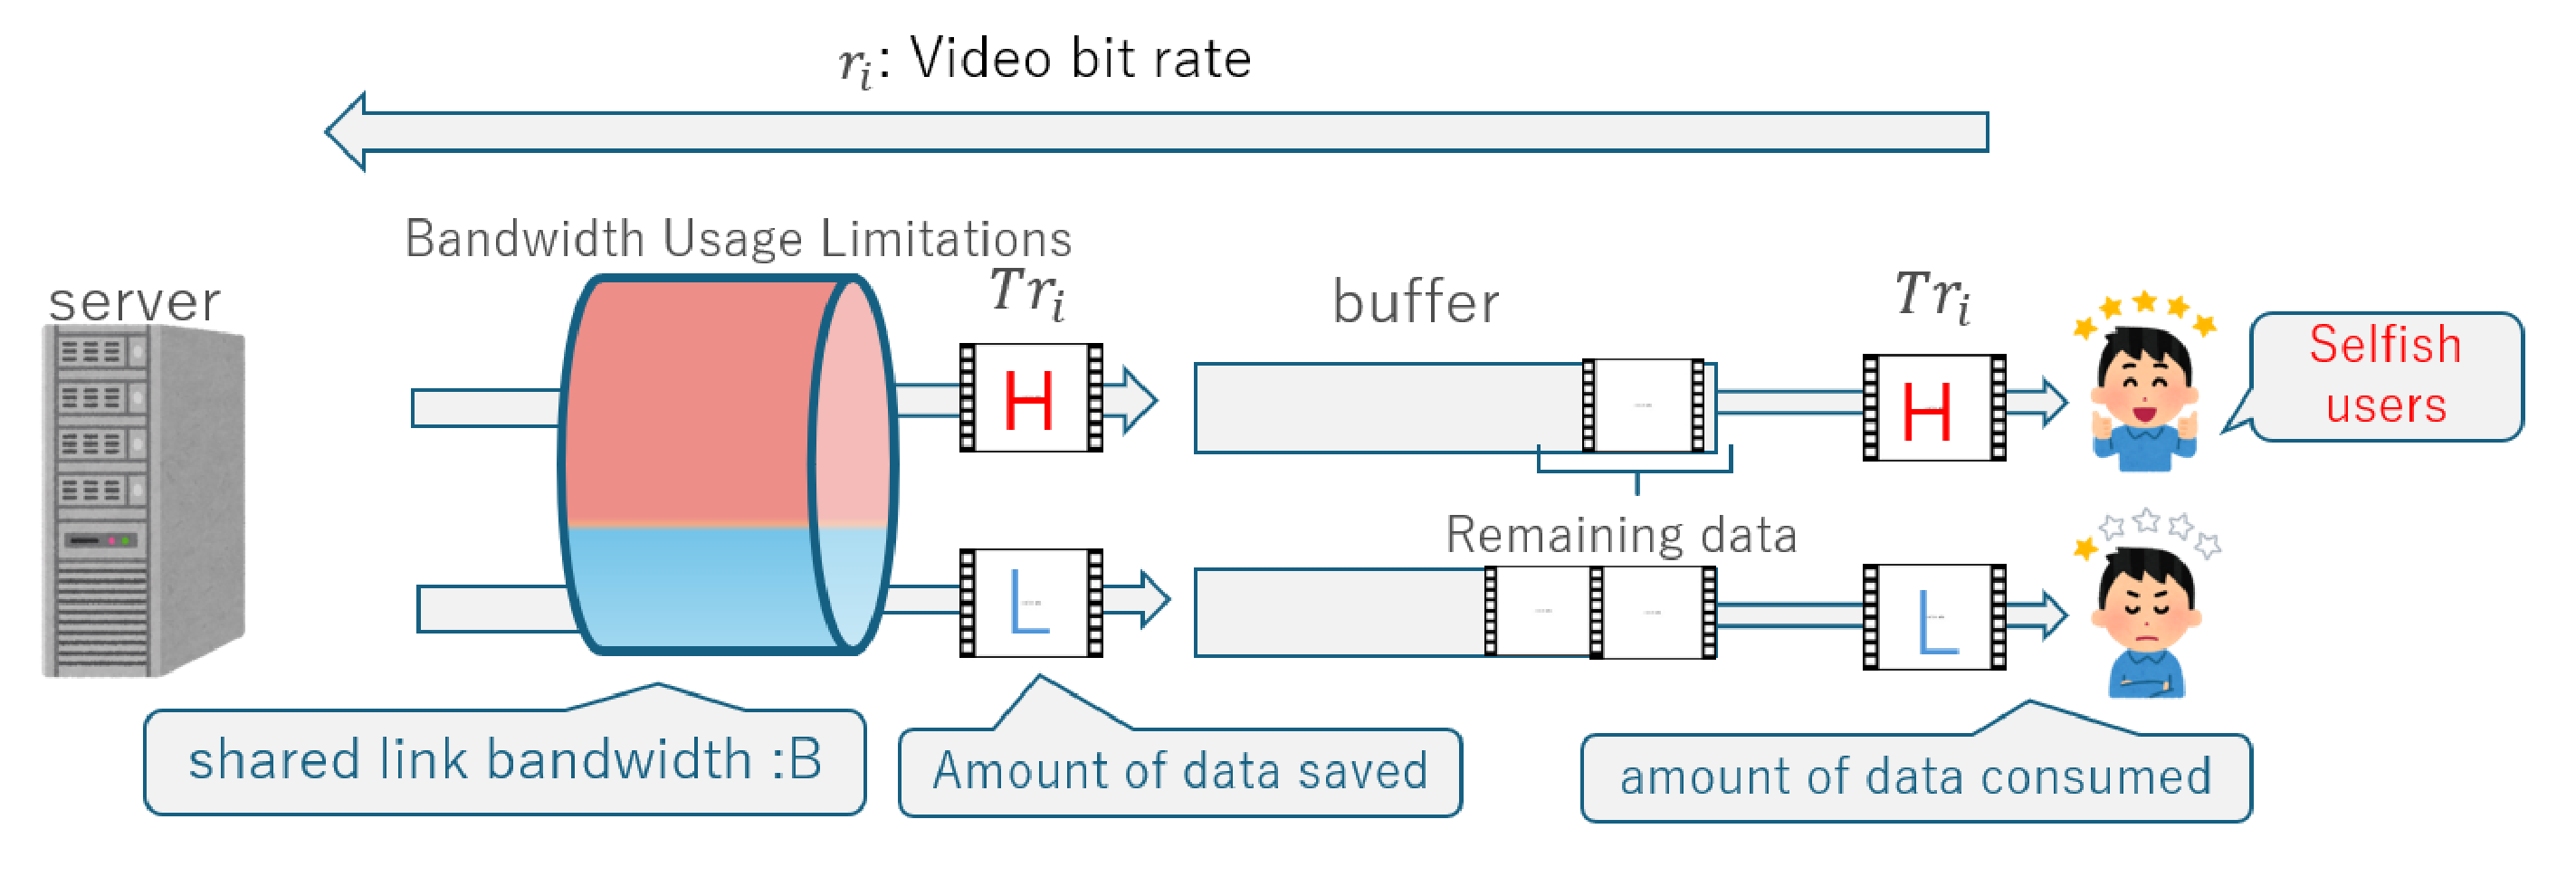
\includegraphics[scale=0.16]{sisutemu.eps}
  \bicaption{想定システム}%
            {Assumed System}
\end{figure}

ゲーム理論を用いることで,共有資源を争うユーザ間の相互依存関係をモデル化し,帯域割り当て問題を解析する.

既存研究\cite{motomoto}では,バッファに蓄積されるデータ量を考慮した利得関数を用いてビデオビットレートを制御している.この利得関数は以下の式で表される.

\begin{equation} 
    f_i=Tr_i-Tr_i\left(\frac{\sum^N_{j=1}r_j}{B}\right) 
\end{equation}

ここで,$T$はセグメント長[s],$N$は全ユーザ数,$r_i$はユーザ$i$のビデオビットレート[Mbps],$B$はリンクの全帯域幅[Mbps]を示す.$\frac{\sum^N_{j=1}r_j}{B}$は,全ユーザの合計使用帯域量を基に各ユーザの平均使用帯域割合を示している.平均使用帯域割合を,各ユーザによる帯域圧迫を考慮し,得られる利得を制限する補正項としている.しかし,この補正項はユーザのビデオビットレート要求が他ユーザの使用帯域に与える影響を反映できていない.

この問題に対し,本研究では次の利得関数への改良を提案する.
 
\begin{equation} 
     f_i=Tr_i-Tr_i\left(\frac{r_i}{B\left(1-\frac{r_i}{\sum^N_{j=1}r_j}\right)}\right) 
\end{equation}

提案する改良法では,ユーザ$i$のビデオビットレートが他ユーザの使用帯域に与える影響を評価する補正項を導入している.$B\frac{r_i}{\sum^N_{j=1}r_j}$
を通じて,ユーザ$i$の使用帯域割合を算出し\cite{johari},補正項である
$\frac{r_i}{B\left(1-\frac{r_i}{\sum^N_{j=1}r_j}\right)}$を導出した.
$\frac{r_i}{B\left(1-\frac{r_i}{\sum^N_{j=1}r_j}\right)}$は,ユーザ$i$のビデオビットレート要求が他ユーザの使用帯域をどの程度圧迫させるかを評価し,得られる利得を制限する.本提案する改良法により,ユーザ毎のビデオビットレート要求による他ユーザの使用帯域への影響を考慮した帯域割り当てが可能となる.





\section{数値計算}
本研究では,数値解析を通じて提案する改良法の有効性を検証した.解析条件として,ユーザ数を2人,セグメント長を$T=1$[s],全帯域幅を$B=4$[Mbps],選択可能なビデオビットレートを$r_i=(1,2,3,4,5,6)$[Mbps]と設定した.


\begin{figure}[h]
  \centering
  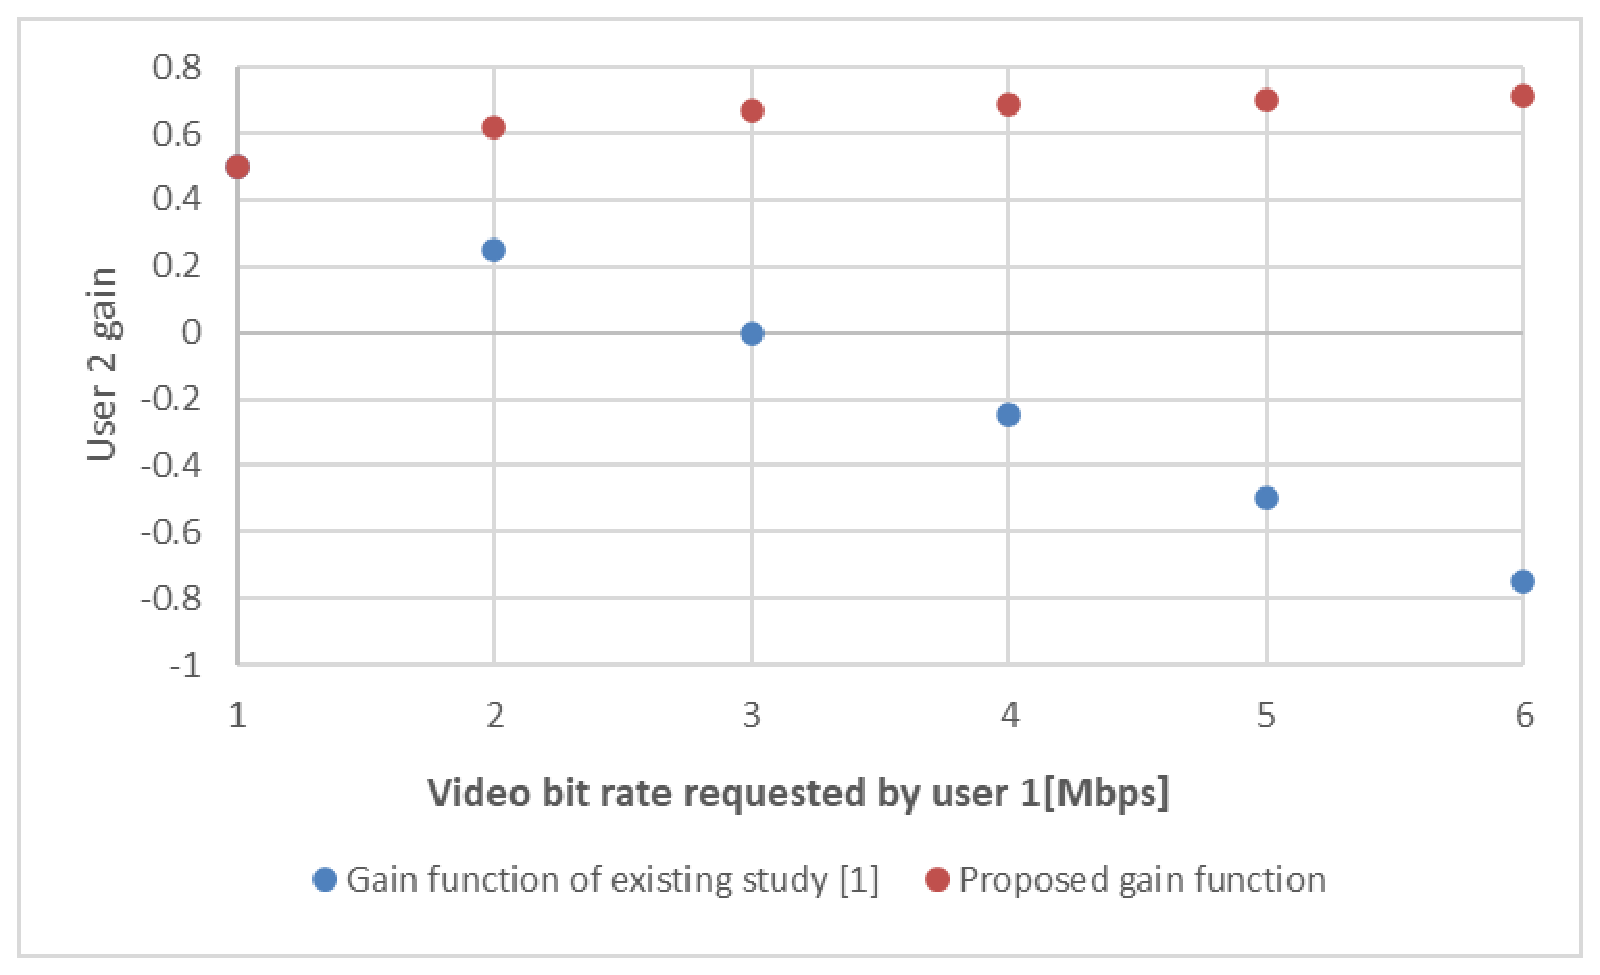
\includegraphics[scale=0.22]{gurahu.eps}
  \bicaption{ユーザ2が1Mbps要求時の利得遷移}%
            {Gain transition when User 2 requests 1 Mbps}
\end{figure}


図2は,ユーザ2のビデオビットレートを1Mbpsに固定し,ユーザ1のビデオビットレートを変化させた際のユーザ2の利得遷移を示している.また,図2で示されるように,既存研究\cite{motomoto}では,ユーザ1のビットレートが増加するにつれ,ユーザ2の利得が大きく減少している.一方,提案した利得関数を用いることで,ユーザ2に対する過渡な制限を回避し,利得の減少を抑制することができた.

これにより,提案する改良法は,各ユーザのビデオビットレートが他ユーザの使用帯域に与える影響を考慮し,特定のユーザへの過渡な利得減少を抑える帯域割り当てを可能にすると言える.


\section{おわりに}
本研究では,ユーザの利己的なビデオビットレート要求が他ユーザの使用帯域に与える影響を考慮した利得関数への改良を提案した.この利得関数により,低ビットレートユーザに対して過渡な制限を課すことなく,各ユーザの影響度に応じた効率的な帯域割り当ての実現性を示した.

今後は,提案した補正項を次のセグメントにおけるビデオビットレート決定に作用させることを検討する.


\section*{参考文献}
\makeatletter
\renewcommand{\section}{\@ifstar{\@section}{}}
\newcommand{\@section}[1]{}
\makeatother
\begin{thebibliography}{99}
    \bibitem{motomoto} H. Yuan, {\it{et al}}., "Non-Cooperative Game Theory Based Rate Adaptation for Dynamic Video Streaming over HTTP," 
IEEE Transactions on Mobile Computing, Vol. 17, No. 10, pp. 2334--2348, Oct. 2018.

    \bibitem{johari} 
K. Sigmund, {\it{et al}}., "Social Learning Promotes Institutions for Governing the Commons," 
Nature, Vol. 466, No. 7308, pp. 861--863, Jul. 2010. 


\end{thebibliography}
\end{document}








##保存
\begin{table}[h]
    \centering
    \caption{新規関数の利得表}
    \scalebox{0.45}{
    \begin{tabular}{|c|c|c|c|c|c|c|}
        \hline
        \diagbox{ユーザ1}{ユーザ2} & 1 & 2 & 3 & 4 & 5 & 6 \\ \hline
        1 & (0.5, 0.5) & (0.62, -1.0) & (0.67, -6.0) & (0.69, -16.0) & (0.7, -32.5) & (0.71, -57.0) \\ \hline
        2 & (-1.0, 0.62) & (0.0, 0.0) & (0.33, -2.62) & (0.5, -8.0) & (0.6, -16.88) & (0.67, -30.0) \\ \hline
        3 & (-6.0, 0.67) & (-2.62, 0.33) & (-1.5, -1.5) & (-0.94, -5.33) & (-0.6, -11.67) & (-0.37, -21.0) \\ \hline
        4 & (-16.0, 0.69) & (-8.0, 0.5) & (-5.33, -0.94) & (-4.0, -4.0) & (-3.2, -9.06) & (-2.67, -16.5) \\ \hline
        5 & (-32.5, 0.7) & (-16.88, 0.6) & (-11.67, -0.6) & (-9.06, -3.2) & (-7.5, -7.5) & (-6.46, -13.8) \\ \hline
        6 & (-57.0, 0.71) & (-30.0, 0.67) & (-21.0, -0.37) & (-16.5, -2.67) & (-13.8, -6.46) & (-12.0, -12.0) \\ \hline
    \end{tabular}
    }
\end{table}

\begin{table}[h]
    \centering
    \caption{既存研究\cite{motomoto}の利得表}
    \scalebox{0.48}{
    \begin{tabular}{|c|c|c|c|c|c|c|}
        \hline
        \diagbox{ユーザ1}{ユーザ2} & 1 & 2 & 3 & 4 & 5 & 6 \\ \hline
        1 & (0.5, 0.5) & (0.25, 0.5) & (0.0, 0.0) & (-0.25, -1.0) & (-0.5, -2.5) & (-0.75, -4.5) \\ \hline
        2 & (0.5, 0.25) & (0.0, 0.0) & (-0.5, -0.75) & (-1.0, -2.0) & (-1.5, -3.75) & (-2.0, -6.0) \\ \hline
        3 & (0.0, 0.0) & (-0.75, -0.5) & (-1.5, -1.0) & (-2.25, -3.0) & (-3.0, -5.0) & (-3.75, -7.5) \\ \hline
        4 & (-1.0, -0.25) & (-2.0, -1.0) & (-3.0, -2.25) & (-4.0, -4.0) & (-5.0, -6.25) & (-6.0, -9.0) \\ \hline
        5 & (-2.5, -0.5) & (-3.75, -1.5) & (-5.0, -3.0) & (-6.25, -5.0) & (-7.5, -7.5) & (-8.75, -10.5) \\ \hline
        6 & (-4.5, -0.75) & (-6.0, -2.0) & (-7.5, -3.75) & (-9.0, -6.0) & (-10.5, -8.75) & (-12.0, -12.0) \\ \hline
    \end{tabular}
    }
\end{table}

% キャプションを「表」に一時的に変更
\renewcommand{\figurename}{表}

\begin{figure}[h]
\centering
\caption{新規関数の利得表}
\vspace{5pt}
\includegraphics[scale=0.24]{sinkiritoku.eps}
\end{figure}

\begin{figure}[h]
\centering
\caption{既存研究の利得表}
\vspace{5pt}
\includegraphics[scale=0.24]{motoritoku.eps}
\end{figure}

%%本研究では,ユーザ$i$の最適画質レート$r_i^*$を決定するため,各ユーザが戦略である画質レートを変更しても利益が増えない状態の戦略の組み合わせ(以降,ナッシュ均衡点と呼ぶ)を求める.ゲーム理論を用いて,$N=\{1,2,3,\dots,n\}$,ユーザ$i$の要求可能画質レートセット$\mathscr{r}_i=\{r^{(1)}_i,r^{(2)}_i,r^{(3)}_i,\dots,r^{(J)}_i\}$,ユーザ$i$の利得関数を$f_i$とし,$G=\left(N,{\mathscr{r}_i}_{(i\in N)},{f_i}_{(i\in N)}\right)$とモデル化する.本研究は,ナッシュ均衡点を利得関数によって決定する.